\section{Problema 2: Centro de Operaciones de Seguridad}

\subsection{Parámetros del SOC}

La Tabla~\ref{tab:soc-parametros} resume los seis escenarios ejecutados. El
caso base usa $\lambda_2=0{,}10$; el Escenario A eleva esa tasa a $0{,}14$
($+40$\,\%). El Escenario B compara $K=16$ con $s=4$ bajo la demanda base y,
como análisis de sensibilidad, bajo la sobrecarga del Escenario A. En todos los
casos $K$ es la capacidad de la cola: la capacidad total es $s+K$.

\begin{table}[H]
\centering
\small
% Tabla generada automáticamente por simulacion_colas.report.
% No editar a mano: regenerar con `python -m simulacion_colas report`.
\begin{tabular}{lrrrrr}
\toprule
Escenario & $s$ & $K$ & $\lambda_2$ (/min) & $\rho_{\text{ofrecida}}$ & Capacidad total \\
\midrule
Base & 3 & 8 & 0,10 & 0,6944 & 11 \\
A (+40\,\%) & 3 & 8 & 0,14 & 0,8389 & 11 \\
B1: $K=16$ & 3 & 16 & 0,10 & 0,6944 & 19 \\
B2: $s=4$ & 4 & 8 & 0,10 & 0,5208 & 12 \\
B1 con sobrecarga A & 3 & 16 & 0,14 & 0,8389 & 19 \\
B2 con sobrecarga A & 4 & 8 & 0,14 & 0,6292 & 12 \\
\bottomrule
\end{tabular}

\caption{Parámetros y carga ofrecida de los escenarios del SOC.}
\label{tab:soc-parametros}
\end{table}

\subsection{Resultados del caso base}

La Tabla~\ref{tab:soc-base} presenta las métricas del caso base con 30
réplicas. La pérdida global es $\loss=0{,}385$\,\%; la de las alertas críticas
es $0{,}431$\,\% y la de las preventivas $0{,}362$\,\%. La utilización conjunta
de los tres analistas es $68{,}87$\,\%, coherente con la carga ofrecida de
$69{,}44$\,\%. Las alertas críticas esperan en promedio $2{,}27$ minutos,
mientras que las preventivas esperan $6{,}42$ minutos: la prioridad no
expropiativa reduce la espera crítica, pero no la elimina porque un servicio
en curso no se interrumpe.

\begin{table}[H]
\centering
\small
% Tabla generada automáticamente por simulacion_colas.report.
% No editar a mano: regenerar con `python -m simulacion_colas report`.
\begin{tabular}{llrrr}
\toprule
Métrica & Unidad & Media & IC95\,\% & Error rel. (\%) \\
\midrule
$W_1$ & min & 22,2603 & [22,2006; 22,3200] & 0,27 \\
$W_{q1}$ & min & 2,2674 & [2,2188; 2,3159] & 2,14 \\
$W_2$ & min & 17,2503 & [17,0634; 17,4372] & 1,08 \\
$W_{q2}$ & min & 6,4171 & [6,2372; 6,5970] & 2,80 \\
$W$ & min & 18,9170 & [18,7786; 19,0555] & 0,73 \\
$W_q$ & min & 5,0367 & [4,9057; 5,1677] & 2,60 \\
$L$ & trabajos & 2,8163 & [2,7871; 2,8456] & 1,04 \\
$L_q$ & trabajos & 0,7502 & [0,7285; 0,7720] & 2,90 \\
$L_{q1}$ & trabajos & 0,1123 & [0,1093; 0,1153] & 2,67 \\
$L_{q2}$ & trabajos & 0,6379 & [0,6182; 0,6576] & 3,09 \\
Utilización & \% & 68,87 & [68,54; 69,20] & 0,48 \\
$P_{\text{loss}}$ & \% & 0,3847 & [0,3372; 0,4323] & 12,35 \\
$P_{\text{loss},1}$ & \% & 0,4306 & [0,3553; 0,5060] & 17,50 \\
$P_{\text{loss},2}$ & \% & 0,3620 & [0,3194; 0,4046] & 11,78 \\
\bottomrule
\end{tabular}

\caption{Métricas del SOC base ($s=3$, $K=8$, $\lambda_2=0{,}10$) con 30 réplicas e IC95\,\%.}
\label{tab:soc-base}
\end{table}

\begin{figure}[H]
\centering
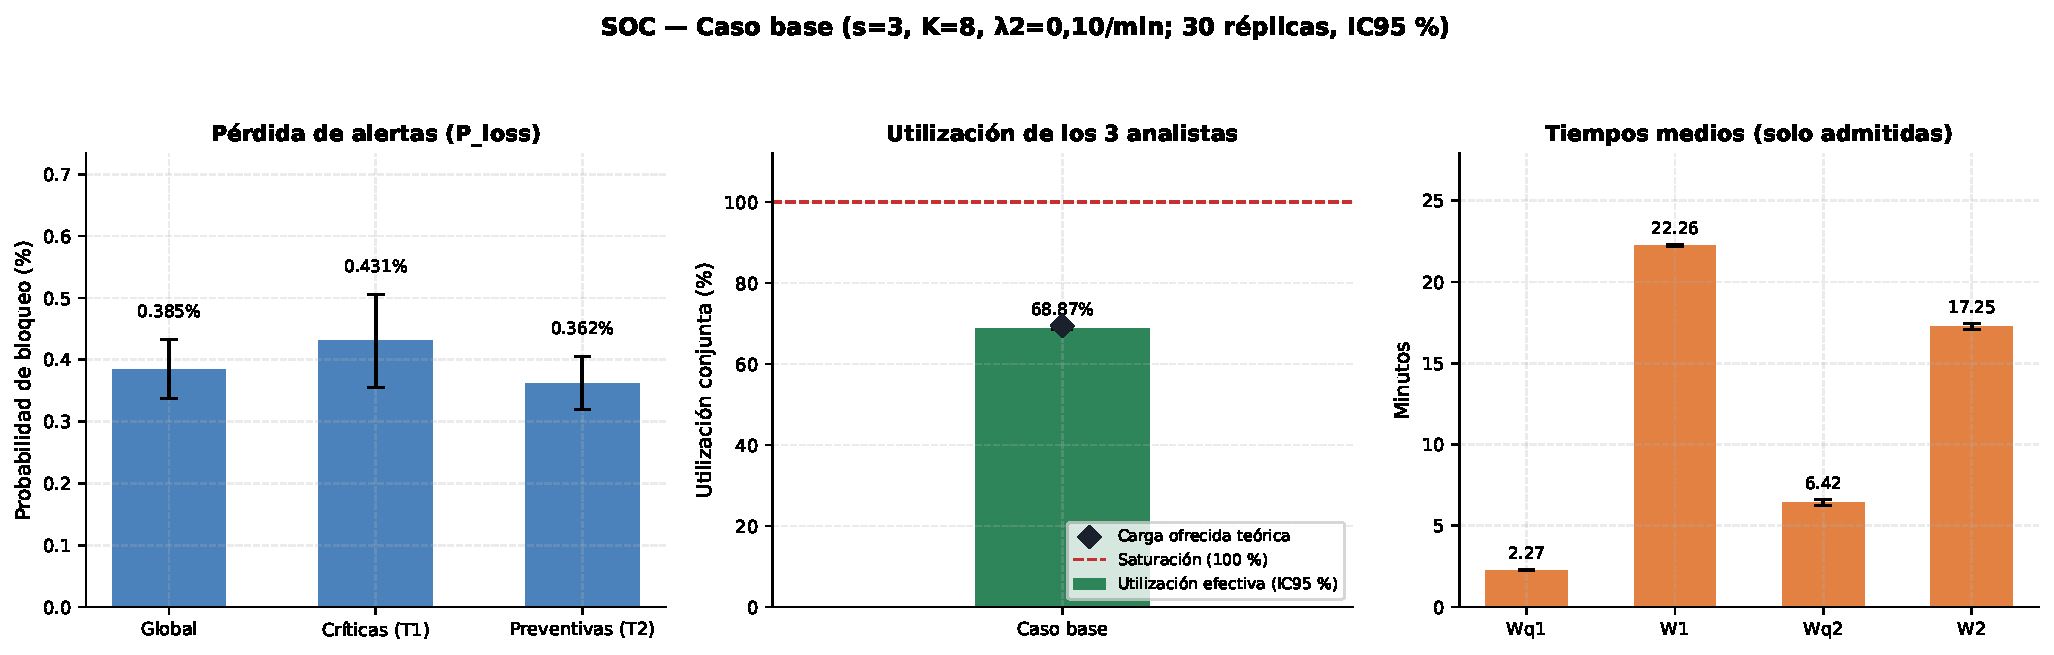
\includegraphics[width=\linewidth]{soc_base.pdf}
\caption{SOC base: probabilidad de bloqueo, utilización y tiempos medios.}
\label{fig:soc-base}
\end{figure}

La Tabla~\ref{tab:conteos} desglosa los conteos medios por tipo de alerta y la
Tabla~\ref{tab:conservacion} verifica las invariantes de conservación en las 30
réplicas. En todas se cumple que las llegadas son iguales a las admitidas más
las bloqueadas, que las admitidas son iguales a las completadas más las
remanentes, y que nunca se superan los tres analistas ni los ocho espacios de
cola.

\begin{table}[H]
\centering
\small
% Tabla generada automáticamente por simulacion_colas.report.
% No editar a mano: regenerar con `python -m simulacion_colas report`.
\begin{tabular}{lrrr}
\toprule
Concepto & Total & Tipo 1 (críticas) & Tipo 2 (preventivas) \\
\midrule
Llegadas & 6455,1 & 2148,3 & 4306,7 \\
Admitidas & 6430,2 & 2139,1 & 4291,1 \\
Bloqueadas & 24,9 & 9,3 & 15,6 \\
Completadas & 6430,2 & 2139,1 & 4291,1 \\
Remanentes al final & 0,0 & 0,0 & 0,0 \\
\bottomrule
\end{tabular}

\caption{Conteos medios por réplica en el SOC base.}
\label{tab:conteos}
\end{table}

\begin{table}[H]
\centering
\small
% Tabla generada automáticamente por simulacion_colas.report.
% No editar a mano: regenerar con `python -m simulacion_colas report`.
\begin{tabular}{lrr}
\toprule
Verificación por réplica & Réplicas que cumplen & Total \\
\midrule
Llegadas $=$ admitidas $+$ bloqueadas & 30 & 30 \\
Admitidas $=$ completadas $+$ remanentes & 30 & 30 \\
Bloqueadas $=$ bloqueadas T1 $+$ T2 & 30 & 30 \\
Admitidas $=$ admitidas T1 $+$ T2 & 30 & 30 \\
Analistas ocupados $\le 3$ y cola $\le 8$ & 30 & 30 \\
\bottomrule
\end{tabular}

\caption{Verificación de invariantes de capacidad y conservación en las 30 réplicas del SOC base.}
\label{tab:conservacion}
\end{table}
